
\documentclass[11pt,a4paper]{article}
\usepackage{graphicx}
\usepackage{float}
\usepackage{titlesec}
\usepackage{fancyhdr}
\pagestyle{fancy}
\setcounter{secnumdepth}{4}
\setcounter{tocdepth}{4}
\fancyfoot[C]{\thepage}
\fancyfoot[L,R]{}
\fancyhead[C]{}
\fancyhead[L]{MChessLink UCI Engine}
\fancyhead[R]{Version 1.3.0}
\title{Millennium ChessLink as UCI Engine}
\author{Lars Nowak}
\date{5 April 2021} 

\begin{document}
\maketitle

\begin{abstract}
The idea is to play with the ChessGenius Exclusive or The King Performance via Millennium ChessLink with all chess GUI’s that support UCI chess engines. The Millennium ChessLink UCI chess engine accepts UCI commands from the GUI and send the chess moves on the board back to the GUI.

I am a professional programmer and write the software in my spare time and it is free. I am not an employee of Millennium 2000 GmbH. If something does not work, Millennium is not responsible for it. On the other hand I cannot guarantee that everything always works, but I try to fix bugs as soon as possible.
\end{abstract}

\newpage
\tableofcontents
\newpage

\section{First of all something technical}

\subsection{Difference between the two zip files}
\begin{itemize}
\item MChessLinkUci.zip\\
This engine based on .NET Framework 4.7.1
\item MChessLinkUciCore.zip\\
This engine based on .NET Core 3.1.0
\end{itemize}
You only need one of them. Both implement the same functionality.
There are some technical reasons in communicating with the hosting GUI to provide two versions. 
If you use HIARCS Chess Explorer, you must use the file MChessLinkUciCore.zip.\\
Because the .NET Core 3.1.0 is still very new, I also provide the other version. You can download .NET Core 3.1.0 runtime on:\\ https://dotnet.microsoft.com/download/dotnet-core/3.1

\subsection{Limitations}

There are some limitations, some of which result from the UCI protocol.
\begin{enumerate}
	\item Some GUIs make their moves from an opening book and inform the engine for the first time for all moves at once when book moves are no longer available. In this case, the GUI must be configured so that at least the MChessLink engine uses its own book.
	\item To play against a real chess engine the GUI must start an engine match where one of the engines is the MChessLink engine.
	\item The communication runs over a device driver witch maps the USB port to a serial port. The driver page of the Millennium Chess Link chipset manufacturer FTDI can be found on: \\ https://www.ftdichip.com/Drivers/VCP.htm
	\\To install the Millennium ChessLink, follow the ChessLink instructions.
\end{enumerate}
\pagebreak

\section{Quick start}
\begin{itemize}
	\item Simply unzip \textbf{one} of the two zip files into a folder. The zip files contain several files.
  
	\item Connect your Millennium ChessLink to your computer and the Millennium chessboard
	\item Set all chessmen to their start position.
	\item Start a GUI (e.g. Fritz, HIARCS Chess Explorer or Arena) and install the MChessLink engine as an UCI engine.
	\item Start an engine match and use MChessLink engine as one of them. Make sure that the GUI configuration allows the engine to use its own opening book.
\end{itemize}


\section{Directories}
After the first start, the engine creates some directories:
\begin{enumerate}
	\item \begin{verbatim}
C:\Users\YOURUSERS\AppData\Local\MChessLinkUci
	\end{verbatim} 
	\item\begin{verbatim}
	C:\Users\YOURUSERS\AppData\Local\MChessLinkUci\log
	\end{verbatim} 
	\item \begin{verbatim}
	C:\Users\YOURUSERS\AppData\Local\MChessLinkUci\engines
	\end{verbatim} 	
		\item \begin{verbatim}
	C:\Users\YOURUSERS\AppData\Local\MChessLinkUci\books
	\end{verbatim} 	
\end{enumerate}
\begin{quote}
YOURUSERS is a placeholder for your Windows user name.
\end{quote}

The first directory contains a configuration file. The second directory contains log files.\\Copy UCI engines into the engines subdirectory to use them in the configuration dialog.\\Copy Polyglot and Arena opening book files into the books subdirectory to use them in the configuration dialog.

\section{Configuration}

\begin{figure}[H]
	\centering
	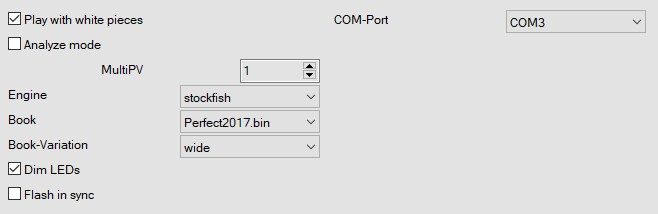
\includegraphics[scale=0.7]{configuration.jpg}
	\caption{Configuration}
	\label{fig:configration}
\end{figure}
\begin{itemize}

	\item \textbf{Play with white pieces} If not checked, you play with the black chessmen and place the black chessmen on the base row (reversed chessboard).

	\item \textbf{MultiPV} Set the number of multiple analyses. This option is only available if there files in the engines directory. This option is ignored on engine matches. With most GUIs this option is not displayed, except for example with Arena.
	
	\item \textbf{Engine} Select one UCI engine located in the engines directory. This option is only available if there files in the engines directory.

    \item \textbf{Analyze mode} Use the selected UCI engine to analyze your moves. This option is only available if there files in the engines directory.
    \item \textbf{Book} Use the selected opening book if you play against an engine. This option is only available if there files in the engines and books directory.
   \item \textbf{Book-Variation} Determine the usage of the book.
   \begin{itemize}
   	  \item \textbf{best move} Always plays the best move.
   	  \item \textbf{flexible} Plays the move considering the weighting or priority.
   	  \item \textbf{wide} Play every move from the book.
   \end{itemize}
    \item \textbf{COM-port} Select an available COM port if automatic detection fails. You can determine or change the correct COM port for the COM device driver in your Windows Device Manager.
    \item \textbf{Dim LEDs} By default the LED's are very bright. They can be darkened using this option.
    \item \textbf{Flash in sync} The source and target fields can flash synchronously or alternately.

\end{itemize}

\subsection{Intention of 'Analyze mode', 'UCI engine' and 'Opening book'}
In most cases it is not necessary or useful to select an UCI engine or opening book in the configuration dialog. Especially \textbf{not} when you are playing an engine match, because you will select your opponent by the GUI.\\The idea behind configuring an UCI engine within the MChessLink engine is to use it in parallel to analyze your moves during the game. For this, select an UCI engine and check the ``Analyze mode`` box. Not to be confused with a post-game analysis, which is provided by most GUI's.\\
Some GUI's allow you to allow an engine to play against itself without initiating a complete engine match. With Arena, for example, you can do this by simply pressing the ``Demo`` button. Now, you can use the MChessLink engine to play against another human being and the GUI is just recording your moves. Or, you configure an UCI engine and play against them in the same simple way. In this case uncheck the ``Analyze mode`` box. To make such a game more variable, you can select an opening book for the UCI engine.\\

\newpage
\section{Use Cases}
The following chapter describes some scenarios and how to manage them in different GUI’s. Please understand that not all GUIs can be considered and some examples are only described for one GUI. I cannot guarantee that all scenarios will work smoothly under all GUI's.
\subsection{Play against another UCI engine}
\subsubsection{Fritz}
\paragraph{Engine Match}
\begin{enumerate}
	\item Start a new engine match.
	\begin{figure}[H]
		\centering
		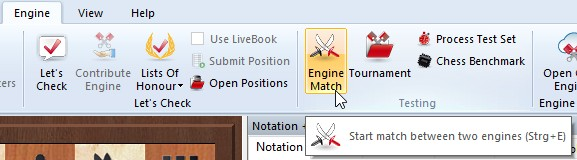
\includegraphics[scale=0.6]{fritz_enginematch.jpg}
		\caption{Fritz Engine Match}
		\label{fig:FritzEngineMatch}
	\end{figure}
	\item Select MChessLink engine for white.
		\begin{figure}[H]
		\centering
		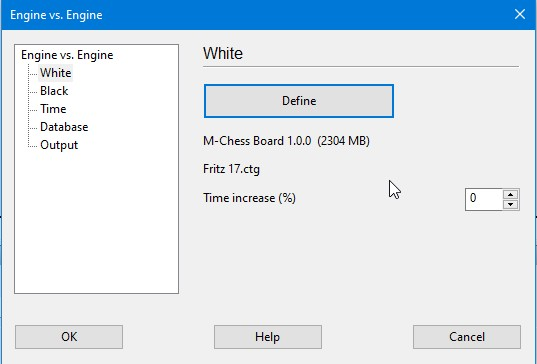
\includegraphics[scale=0.7]{fritz_enginewhite.jpg}
		\caption{Define Engine for White}
		\label{fig:FritzEngineWhite}
	\end{figure}
	\item Open the engine configuration dialog and uncheck ``Analyze mode`` and select ``\begin{math}<none>\end{math}`` as UCI engine.
			\begin{figure}[H]
		\centering
		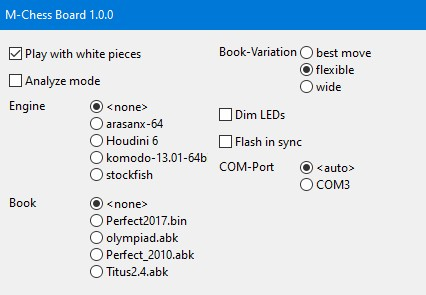
\includegraphics[scale=0.8]{fritz_engine_configure_mchesslink.jpg}
		\caption{Configure MChessLink Engine}
		\label{fig:FritzConfigureCertabo}
	\end{figure}

	\item Ensure the checkbox for ``Use book`` is unchecked.
		\begin{figure}[H]
		\centering
		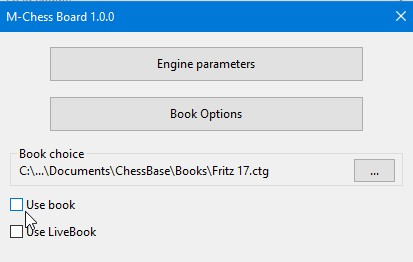
\includegraphics[scale=0.8]{fritz_engineusebook.jpg}
		\caption{Use Book}
		\label{fig:FritzUseBook}
	\end{figure}
	\item Select an engine installed in Fritz for black.
	\item Set your preferred time settings and start the match.	
\end{enumerate}

\subsubsection{Arena}
Arena allows different ways to play against another UCI engine. It is common that the MChessLink UCI engine must not use the Arena opening book. Deactivate the option ``Use Arena general main books with this engine``.
\begin{figure}[H]
	\centering
	\includegraphics[scale=0.7]{arena_mainbooks.jpg}
	\caption{MChessLink Arena Book}
	\label{fig:ArenaUseBook}
\end{figure}
\paragraph{With one MChessLink engine and one UCI Engine}
\begin{enumerate}
\item Load MChessLink engine as \mbox{``Engine 1``} and the opponent UCI engine as \mbox{``Engine 2``}.
	\begin{figure}[H]
	\centering
	\includegraphics[scale=0.7]{arena_engine1.jpg}
	\caption{MChessLink UCI as Engine 1}
	\label{fig:ArenaEngine1}
\end{figure}
\item Configure Engine 1 (MChessLink engine)
\begin{figure}[H]
	\centering
	\includegraphics[scale=0.6]{arena_configureengine1.jpg}
	\caption{Configure Engine 1}
	\label{fig:ArenaConfigureEngine1}
\end{figure}
\item Open the engine configuration dialog and uncheck ``Analyze mode`` and select ``\begin{math} <none> \end{math}`` as UCI engine.
\begin{figure}[H]
	\centering
	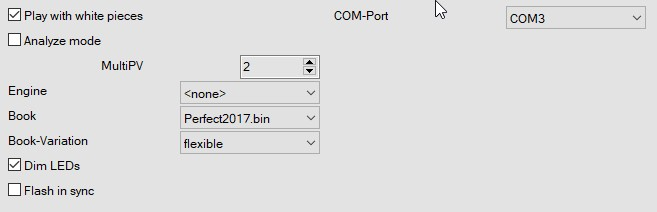
\includegraphics[scale=0.7]{Arena_ConfigureMChessLink.jpg}
	\caption{Configure MChessLink Engine}
	\label{fig:ArenaConfigureCertabo}
\end{figure}
\item Press ``Demo`` to start the game.
\begin{figure}[H]
	\centering
	\includegraphics[scale=0.7]{arena_demo.jpg}
	\caption{Run Demo}
	\label{fig:ArenaDemo}
\end{figure}
\end{enumerate}

\paragraph{With one MChessLink engine}
\subparagraph{} If you have copied an UCI engine into the engine subfolder, you can use them as opponent.
\begin{enumerate}
	\item Close ``Engine 2`` if loaded.
	\begin{figure}[H]
		\centering
		\includegraphics[scale=0.7]{arena_closeengine2.jpg}
		\caption{Close Engine 2}
		\label{fig:ArenaCloseEngine2}
	\end{figure}
    \item Open the MChessLink engine configuration dialog and uncheck ``Analyze mode`` and select an UCI engine and an opening book if available.
    	\begin{figure}[H]
    	\centering
    	\includegraphics[scale=0.7]{arena_ConfigureMChessLink2.jpg}
    	\caption{Select an UCI Engine}
    	\label{fig:ArenaConfigureCertabo2}
    \end{figure}
    \item Press ``Demo`` to start the game.
    \begin{figure}[H]
    	\centering
    	\includegraphics[scale=0.7]{arena_demo.jpg}
    	\caption{Run Demo}
    	\label{fig:ArenaDemo}
    \end{figure}
\end{enumerate}

\paragraph{Engine Tournament}
\begin{enumerate}
\item Start an Engine Tournament
  \begin{figure}[H]
	\centering
	\includegraphics[scale=0.7]{arena_enginetournament.jpg}
	\caption{Arena Engine Tournament}
	\label{fig:ArenaEngineTournament}
\end{figure}
\item For the MChessLink engine make sure that ``Analyze mode`` is unchecked and  ``\begin{math} <none> \end{math}`` as the selected UCI engine.
\end{enumerate}
You can add the MChessLink engine twice with different names. So, you can play a tournament against yourself with different configurations, e.g. different UCI engines for analysis.

\subsection{Use an UCI engine for analysis}
In this case, the UCI engine shows you the analysis for your moves during the game. Opening books will be ignored.
\subsubsection{Fritz}
\paragraph{Engine Match}
\begin{enumerate}
	\item Start a new engine match.
	\begin{figure}[H]
		\centering
		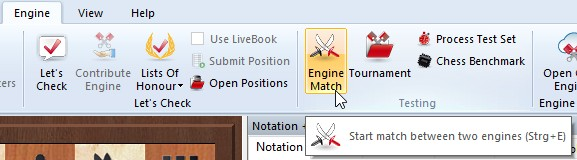
\includegraphics[scale=0.6]{fritz_enginematch.jpg}
		\caption{Fritz Engine Match}
		\label{fig:FritzEngineMatch}
	\end{figure}
	\item Select MChessLink engine for white.
	\begin{figure}[H]
		\centering
		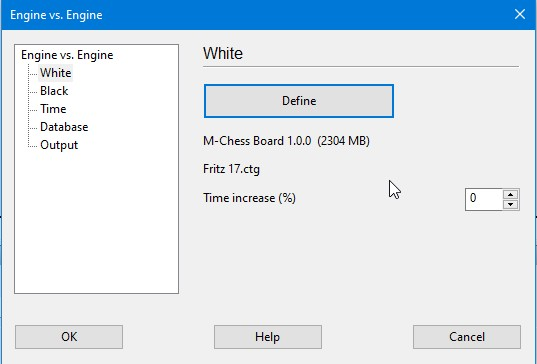
\includegraphics[scale=0.6]{fritz_enginewhite.jpg}
		\caption{Define Engine for White}
		\label{fig:FritzEngineWhite}
	\end{figure}
	\item Open the engine configuration dialog and check ``Analyze mode`` and select an UCI engine.
	\begin{figure}[H]
		\centering
		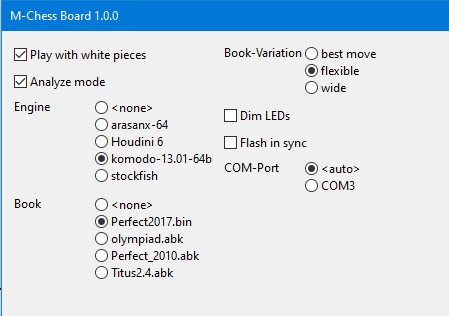
\includegraphics[scale=0.8]{fritz_engine_configure_mchesslink_analyze.jpg}
		\caption{Configure MChessLink Engine}
		\label{fig:FritzConfigureCertabo}
	\end{figure}
	
	\item Ensure the checkbox for ``Use book`` is unchecked.
	\begin{figure}[H]
		\centering
		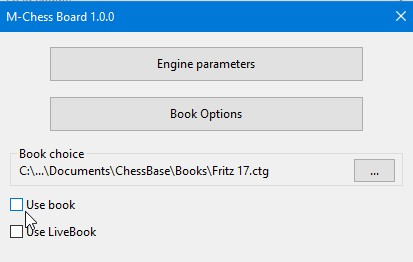
\includegraphics[scale=0.6]{fritz_engineusebook.jpg}
		\caption{Use Book}
		\label{fig:FritzUseBook}
	\end{figure}
	\item Select an engine installed in Fritz for black.
	\item Set your preferred time settings and start the match.	
\end{enumerate}
\subsubsection{Arena}
You can play an engine match like described above with Fritz but you can use the ``Demo`` mode, too. In Arena you can install the same engine with different parameters under a new name. So, you can play an engine match with two MChessLink engines as opponent with different UCi engines for analysis. Arena allows you, a little bit aside by the UCI protocol definition, to configure the MultiPV-Parameter for an engine match. This gives you the possibility to display several analysis lines during the games.

\subsection{Start from a position}
You can start from any chess position specified by the GUI. It is best to place the chessmen first on your MChessLink chessboard and then use the setup position functionality of your GUI.
\subsubsection{Arena}
\begin{enumerate}
  \item Open the Set-up Position dialog and place the chessmen.
  \item Close the dialog and press the demo button. The chessboard LED indicate incorrectly placed or missing chessmen.
\end{enumerate}

\section{Important To Know}
\subsection{Log files}
The MChessLink engine writes at least two log files into the log directory:
\begin{enumerate}
  \item mchesslinkUci\_1.log
  \item mchesslink\_1.log
\end{enumerate}
If the GUI starts a second instance of the engine, e.g. you start an engine match against two MChessLink UCI engines, the log files for the second engine are named mchesslinkUCi\_2.log and mchesslink\_2.log.


\subsection{COM port}
The engine detects all available COM ports and uses the first one found. If you set another COM port on the configuration, you may have to restart the engine to activate it.

\subsection{Opening books}
The engine supports Polyglot and Arena opening books. The internal data structure of both are very different. In simple words, Polyglot is position oriented and Arena move oriented. You can use a Polyglot opening book for normal game or from any starting position. If you use an Arena opening book, the engine will not find the next move unless you start from the beginning of a game.

\section{Trouble shooting}


\subsection{The chess moves are not or not correctly displayed}
\begin{itemize}
	\item Check the correct COM port in the configuration dialog.
	\item Check the position of the chessmen. Moves are only accepted if the chessmen are on the correct square. Fields with missing or wrong figure light up.
	\item Try the engine from the MChessLinkUciCore.zip file.
	\item Finally, the UCI protocol is well defined but not every GUI send the commands in the same way. I test the engine with the common used GUI's but may some are different.
\end{itemize}

\subsection{The engine makes the moves itself}
\begin{itemize}
\item If you are playing an engine match, open the configuration dialog and select the option ``Analyze mode`` or set the UCI engine to ``\begin{math}<none>\end{math}``.
\item Make sure that the GUI does not make the moves by using an opening book.
\end{itemize}

\section{Known Issues}
\begin{itemize}
    \item Sometimes your moves are not recognized on the chessboard. Just repeat them. This mostly happens if you move to fast.
	\item When no more moves are found in the opening book for the first time, the system no longer looks in the book for that game.
\end{itemize}

\section{Next Steps}
\begin{itemize}
	\item Improving the COM port detection.
	\item Improving the chess move detection.
	\item Error correction.
\end{itemize}

\pagebreak

\section{Changelog}
\subsection{Version 1.2.0 =\textgreater 1.3.0}
\begin{itemize}
	\item Improvement of the COM port detection.
\end{itemize}
\subsection{26 July 2020 =\textgreater Documentation revised}
\subsection{Version 1.1.2 =\textgreater 1.2.0}
\begin{itemize}
	\item Great improvement in the recognition of chess moves.
\end{itemize}
\subsection{Version 1.1.1 =\textgreater 1.1.2}
\begin{itemize}
	\item Important bug fix for long castling. The rook was internally set to an invalid square.
\end{itemize}
\subsection{Version 1.1.0 =\textgreater 1.1.1}
\begin{itemize}
	\item Bug fixing .Net Core
\end{itemize}
\subsection{Version 1.0.1 =\textgreater 1.1.0}
\begin{itemize}
	\item Bug fixing on LED for field D5.
    \item Better detection when the chessmen are moved slowly over the bed.
    \item By refactoring the code more DLL files have been created.
\end{itemize}
\subsection{Version 1.0.0 =\textgreater 1.0.1}
\begin{itemize}
	\item Bug fixing on configure COM port.
\end{itemize}
\end{document}